\documentclass[twoside,12pt,openright,AutoFakeBold]{ctexbook}

%======================= 宏包加载(正文相关) ===========================
\usepackage{wallpaper}     % 封面背景
\usepackage{amsmath,mathtools,amsthm,amsfonts,amssymb,bm}  % AMS 数学宏包
\usepackage{color}         % 支持颜色设置
\usepackage{fontspec}      % 字体设置(适用于 XeLaTeX)
\usepackage{setspace}      % 行距设置
\usepackage{indentfirst}   % 首段缩进
\setlength{\parindent}{2em}

%======================= 页面设置 ===========================
\usepackage{geometry}      % 页面边距设置
\geometry{
    a4paper,
    inner=45mm,
    outer=20mm,
    top=25mm,
    bottom=20mm, % 添加底部页边距
    %textheight=244mm,
    headheight=21.7mm
}

%======================= 页眉页脚设置 ===========================
\usepackage{fancyhdr}      % 自定义页眉页脚
\fancypagestyle{myfancy}{
    \fancyhf{}  % 清空原有设置
    \fancyfoot[CE,CO]{\thepage}
    \fancyhead[CE]{\songti\zihao{5}西北大学本科毕业论文(设计)}
    \fancyhead[CO]{\nouppercase{\leftmark}}
    \renewcommand{\headrule}{
        \makebox[0pt][l]{\rule[.7\baselineskip]{\headwidth}{3pt}}%
        \rule[.6\baselineskip]{\headwidth}{0.4pt}\vskip-.8\baselineskip
    }
}

%======================= 脚注设置 ===========================
\usepackage{pifont}        % 用于 \ding 圆圈数字
\usepackage{alphalph}      % 脚注编号扩展
\usepackage{chngcntr}      % 编号控制
\counterwithout{footnote}{chapter}  % 脚注全局编号
\newcommand{\circled}[1]{\ding{\numexpr171 + #1\relax}}
\renewcommand{\thefootnote}{\protect\circled{\value{footnote}}}

%======================= 标题格式设置 ===========================
\ctexset{
    chapter = {
        name = {},
        number = 第\Chinese{chapter}章,
        format += {\heiti\zihao{-2}\centering},
        beforeskip = 36pt,
        afterskip = 24pt,
        fixskip = true
    },
    section = {
        format += {\heiti\zihao{4}\raggedright},
        beforeskip = 18pt,
        afterskip = 18pt
    },
    subsection = {
        format += {\heiti\zihao{-4}\raggedright},
        beforeskip = 12pt,
        afterskip = 12pt
    }
}

%======================= 目录格式设置 ===========================
\usepackage{titletoc}
\renewcommand{\contentsname}{\heiti \zihao{-2}目\quad 录}

\titlecontents{chapter}[3em]
    {\vspace*{7pt}\heiti\zihao{4}}
    {\contentslabel{3.5em}}
    {\hspace*{-3.4em}}
    {~\titlerule*[0.6pc]{$.$}~\zihao{-4}\contentspage}

\titlecontents{section}[4em]
    {\songti\zihao{-4}}
    {\contentslabel{2em}}
    {\hspace*{-2em}}
    {~\titlerule*[0.6pc]{$.$}~\contentspage}

\titlecontents{subsection}[6em]
    {\songti\zihao{-4}}
    {\contentslabel{3em}}
    {\hspace*{-2em}}
    {~\titlerule*[0.6pc]{$.$}~\contentspage}

%======================= 参考文献设置 ===========================
\usepackage[
    backend=biber,
    style=gb7714-2015,
    sorting=none
]{biblatex}
\addbibresource{bib/ref.bib}

%======================= 定理环境定义 ===========================
\newtheoremstyle{mydefstyle}
  {1em}{1em}{}{}{\heiti \zihao{-4}}{.}{1em}{}
\theoremstyle{mydefstyle}

\newtheorem{definition}{\hskip 2em{定义}}[section]
\newtheorem{theorem}{\hskip 2em{定理}}[section]
\newtheorem{assumpation}[theorem]{\hskip 2em{假设}}
\newtheorem{lemma}[theorem]{\hskip 2em{引理}}
\newtheorem{corollary}[theorem]{\hskip 2em{推论}}
\newtheorem{example}{\hskip 2em{算例}}[chapter]
\newtheorem{remark}{\hskip 2em{注}}[chapter]
\renewcommand{\proofname}{\bf 证明}

%======================= 图表设置 ===========================
\usepackage{bicaption}
\captionsetup[figure][bi-second]{name=Fig}
\captionsetup[table][bi-second]{name=Table}

%======================= 数学符号与公式编号 ===========================
\renewcommand{\Re}{\operatorname{Re}}
\renewcommand{\Im}{\operatorname{Im}}
\newcommand{\mi}{\mathrm{i}}
\newcommand{\md}{\mathrm{d}}
\newcommand{\me}{\mathrm{e}}
\allowdisplaybreaks[4]
%\numberwithin{equation}{section} % 若需要按章节编号

%======================= 列表设置 ===========================
\usepackage[inline]{enumitem}
\setlist{
    topsep=0.3em,
    partopsep=0pt,
    itemsep=0ex plus 0.1ex,
    parsep=0pt,
    leftmargin=1.5em,
    rightmargin=0em,
    labelsep=0.5em,
    labelwidth=2em
}

%======================= 图像与表格 ===========================
\usepackage{graphicx,ragged2e}
\usepackage{subcaption}
\graphicspath{figure/}
\usepackage{longtable,booktabs}

%======================= 代码环境 ===========================
\usepackage{listings}
\renewcommand{\lstlistingname}{算法}
\lstset{
    keywordstyle=\bfseries,
    basicstyle=\ttfamily,
    commentstyle=\ttfamily,
    showstringspaces=false,
    breaklines=true,
    frame=single
}

%======================= 超链接设置 ===========================
\usepackage{hyperref}
\hypersetup{
    colorlinks=true,
    urlcolor=black,
    linkcolor=black,
    anchorcolor=black,
    citecolor=black
}

%======================= 插入 PDF ===========================
\usepackage[final]{pdfpages}

%======================= 正文开始 ===========================
\begin{document}

%========= 前置部分 =========
\frontmatter
\pagestyle{empty}
% -*- coding=utf-8 -*-   % 指定文件编码为 UTF-8,确保中文正常显示

%\newcommand\clcNumber{O175.3}    % 分类号(可选),如不需要可注释掉
                                  % 二级学科名称(此处为空,可自行添加)
\newcommand\addtion{教务处制}     % 附加说明,通常为制表单位
\newcommand{\thesisTitle}{XXXX}   % 论文标题
\newcommand{\thesisAuthor}{XX}    % 学生姓名
\newcommand{\studentId}{xxxxxxxx} % 学号
\newcommand{\supervisor}{xxxxx}   % 指导教师姓名
\newcommand{\institute}{xx学院}   % 学院名称
\newcommand{\major}{xxxxxx}       % 专业名称
\newcommand{\grade}{xxxxx}        % 年级

% ============================= 封面页面设置(如有必要可自行更改) =============================

% 封面背景为已导出的 PDF 文件(建议封面背景图为无白边且对齐的 PDF)
{
    \setlength\parindent{0em} % 取消首行缩进
    \ThisTileWallPaper{\paperwidth}{\paperheight}{figure/nwucover.pdf} % 设置封面背景图片
    \vspace*{0.2cm} % 设置页面内容的上边距

    \vspace*{9.5cm} % 控制标题区域的垂直位置

    % ============================= 论文标题设置 =============================
    % 如果标题较短,可使用以下单行写法(已注释):
    % \begin{center}
    %     \zihao{3}  题目:\underline{\makebox[9cm][c]{\heiti\zihao{2}\thesisTitle}}
    % \end{center}

    % 如果标题较长,可使用如下分两行写法(当前启用):
    \begin{center}
        {\zihao{3}  题目:}   \underline{\makebox[22em][c]{\zihao{2}\heiti 我的本科毕业论文题目}} \par
        {\zihao{-3} \qquad\quad }   \underline{\makebox[22em][c]{\zihao{2}\heiti 实在是太长了 }} \par
    \end{center}

    \vspace{0.4cm} % 控制标题与学生信息之间的垂直间距

    \renewcommand{\baselinestretch}{2.25}\selectfont % 设置行间距

    % ============================= 学生信息区域 =============================
    {
        \begin{center}
        \songti % 设置字体为宋体
        {\zihao{-3} 学生姓名} \underline{\makebox[10em][c]{\zihao{-3}\thesisAuthor}} \par
        {\zihao{-3} 学\;\;\;\;\;\;\;号} \underline{\makebox[10em][c]{\zihao{-3}\studentId}} \par
        {\zihao{-3} 指导教师} \underline{\makebox[10em][c]{\zihao{-3}\supervisor}} \par
        {\zihao{-3} 院\;\;\;\;\;\;\;系} \underline{\makebox[10em][c]{\zihao{-3}\institute}} \par
        {\zihao{-3} 专\;\;\;\;\;\;\;业} \underline{\makebox[10em][c]{\zihao{-3}\major}} \par
        {\zihao{-3} 年\;\;\;\;\;\;\;级} \underline{\makebox[10em][c]{\zihao{-3}\grade}} \par
        \end{center}
    }
}
 %封面

\includepdf[pages={1}]{figure/Declaration.pdf} %诚信声明
\pagestyle{plain}
\pagenumbering{Roman}
\let\cleardoublepage\clearpage
% -*- coding=utf-8 -*-

%
\chapter*{\heiti\zihao{-2}摘\ \ \  要} % 使用星号形式,不自动添加到目录
\addcontentsline{toc}{chapter}{摘要} % 手动添加目录项,使用默认字体字号
\begin{spacing}{1.66}
{\songti\zihao{-4}\selectfont

\begin{center}
十六字令三首

毛泽东

山,快马加鞭未下鞍。惊回首,离天三尺三。

山,倒海翻江卷巨澜。奔腾急,万马战犹酣。

山,刺破青天锷未残。天欲堕,赖以拄其间。
\end{center}
}
\end{spacing}

\heiti\zihao{-4}关键词:\songti\zihao{-4}山;山;山
%关键词:按与论文内容紧密程度依次列出 3-5 个关键词。
\clearpage	
% 跳到目录下一页
%\thispagestyle{plain}						% 显示最后一页的页码
%中文摘要:在主体内容前用 200-300 字的中文扼要介绍论文的主要内容、采用的研究方法和得到的主要结论。 %中文摘要
\cleardoublepage
% -*- coding=utf-8 -*-
\chapter*{\fontsize{18}{24}\selectfont \textbf{ABSTRACT}} % 使用星号形式,不自动添加到目录
%粗体小二18pt
\addcontentsline{toc}{chapter}{Abstract} %
\setmainfont{Times New Roman} % 设置英文字体
\begin{spacing}{1.66}
\zihao{-4}\selectfont

\begin{center}
\Large \textbf{Three Verses of the Sixteen-Character Poem} \\
\large by Mao Zedong
\end{center}

\vspace{1em}

\begin{center}
\textbf{1} \\
Mountains— \\
Whip the horse, the saddle stays; \\
Startled, I glance back— \\
The sky is but three feet away. \\
\end{center}

\vspace{1em}

\begin{center}
\textbf{2} \\
Mountains— \\
Oceans overturned in roaring waves. \\
Gallop they go, \\
Ten thousand steeds in warlike craze. \\
\end{center}

\vspace{1em}

\begin{center}
\textbf{3} \\
Mountains— \\
Pierce the blue heavens with blade unfrayed. \\
Should the sky fall, \\
It is they who bear its weight. \\
\end{center}



\end{spacing}

\zihao{-4}\textbf{Key words: }\zihao{-4} Mountains;Mountains;Mountains

\clearpage									% 跳到目录下一页
%\thispagestyle{plain}						% 显示最后一页的页码
%英文摘要与关键词:内容与中文摘要相同。最后一行注明论文的关键词(3-5 个)。 %英文摘要


%========= 目录部分 =========
\pagestyle{plain}
\setcounter{page}{1}
\pagenumbering{Roman}
\tableofcontents
\clearpage
\thispagestyle{plain}

%========= 正文部分 =========
\mainmatter
\fancypagestyle{plain}{\pagestyle{myfancy}}
\pagestyle{myfancy}
% -*- coding=utf-8 -*-
% 教程:按照给出的例子编辑tex/chapters目录下的文件,然后注释掉What is it和writeExample这两个示例章节即可。
% -*- coding=utf-8 -*-
\chapter{引言}   % \chapter{短标题}{长标题} 页眉会显示短标题,正文会显示长标题,“\\"会强制换行,”\ “会显示空格
\songti\zihao{-4}
\linespread{1.67} \selectfont       % 导入章节一
% -*- coding=utf-8 -*-
\chapter{预备知识}   % \chapter{短标题}{长标题} 页眉会显示短标题,正文会显示长标题,“\\"会强制换行,”\ “会显示空格
\songti\zihao{-4}
\linespread{1.67} \selectfont       % 导入章节二
% -*- coding=utf-8 -*-
\chapter[基础]{基础}  % \chapter[短标题]{长标题} 页眉会显示短标题,正文会显示长标题,“\\"会强制换行,”\ “会显示空格题目:要体现专业特点,应精练、准确地概括论文研究的主要内容和结果,一般不超过 20 字。
\songti\zihao{-4}
\linespread{1.67} \selectfont

本模板为西北大学学士学位论文的 \LaTeX 排版示例,参考自\href{https://www.overleaf.com/latex/templates/shan-xi-shi-fan-da-xue-li-gong-ke-lei-ben-ke-sheng-bi-ye-lun-wen-texmo-ban/rkxzpttqqzyt}{\color{red}{陕西师范大学本科生毕业论文模板}},并依据学校提供的论文写作规范进行了适当修改与优化。如模板中存在不符合个人或学校实际要求之处,可根据需要自行调整。

\section{文档说明}

\subsection{准备工作}

在 \textbf{\textcolor{green}{Overleaf}} 平台上使用本模板时,只需在菜单栏中将编译器设置为 \textbf{\textcolor{green}{XeLaTeX}},即可正常编译运行。

若在本地使用,需先安装 \textbf{\textcolor{green}{TeX Live 2024}} 作为编译环境,并选择合适的编辑器(如 \textbf{\textcolor{green}{TeXstudio}} 或 \textbf{\textcolor{green}{Visual Studio Code}})。安装方法可参考互联网资源(如 \textbf{\textcolor{green}{Bilibili}}、\textbf{\textcolor{green}{CSDN}}、\textbf{\textcolor{green}{博客园}}等),或选择在 \textbf{\textcolor{green}{淘宝}}、\textbf{\textcolor{green}{京东}} 等平台寻求远程安装服务。

\subsection{编译方法}

在 \textbf{\textcolor{green}{Overleaf}} 中,点击“编译”按钮即可完成编译。

在本地使用 \textbf{\textcolor{green}{VS Code}} 时,若仅需快速编译正文而不更新参考文献,可直接选择 \textbf{\textcolor{green}{XeLaTeX}} 编译,以加快速度;若需要重新生成参考文献,则应选择 \textbf{\textcolor{green}{XeLaTeX \& Biber}} 编译方式。


\section{模板文件结构}

本节介绍模板的文件结构,该模板采用配置与内容分离的设计,主要包含根目录下的配置文件main.tex以及三个子目录bib,figure,tex。

如果想要修改全局的配置,就去main.tex;
想要编辑论文的内容,就去tex/目录;
图片都放到figure/目录;
参考文献数据放在bib/目录。

\subsection{配置文件main.tex}

配置文件main.tex的作用在于定义全局配置,例如文档类型,引入宏包,页面布局等,可以理解为tex文件的导言区。

\subsection{内容目录tex/}

tex目录下共有九个文件tex文件,分别对应于封面,原创性声明页,中文摘要,英文摘要,正文页,总结页,参考文献,致谢,研究成果页。此外还有一个子目录chapters/用来存放正文页导入的内容。

封面页只需要修改最开始的几个参数即可。

原创性声明页一般无需改动。

中文摘要,英文摘要,正文页,总结页,致谢需要自行编辑。

研究成果页已经给出了示例,仿造一下即可。

\subsection{参考文献目录bib/}

目录下有一个参考文献数据库文件\verb|ref.bib|来存放学位论文参考的文献信息。

\subsection{图片目录figure/}

存放需要用到的图片,本模板可以使用的格式包括pdf,jpg,png,eps。
配置文件中已经定义了图片的存放路径,所以插入图片的时候,顶层目录figure/可以省略。作者建议不要省略,可读性更强一些。

% -*- coding=utf-8 -*-
\chapter{写作示例}

\section{列表环境}

\subsection{无序列表}

使用环境\verb+itemize+是一个无序列表的例子,列表的每个条目单独分段。

\begin{itemize}
	\item 这是一个无序列表。
	\item 这是一个无序列表。
	\item 这是一个无序列表。
\end{itemize}

\subsection{有序列表}

使用环境\verb+enumerate+创建有序列表,使用方法与无序列表类似。

\begin{enumerate}[label={\arabic*}]
	\item 这是一个有序列表。
	\item 这是一个有序列表。
	\item 这是一个有序列表。
\end{enumerate}

通过修改\verb+enumerate+环境后的参数\verb+[label={\arabic*}]+可以实现编号数字类型的切换。
\verb+\arabic+可以替换为\verb+\roman+,\verb+\Roman+,\verb+\alph+,\verb+\Alph+来表示小写罗马数字,大写罗马数字,小写字母编号,大写字母编号。

可以加入一些括号让列表更加好看,例如:\verb+[label={\roman*)}]+显示效果如下

\begin{enumerate}[label={\roman*)}]
	\item 这是一个有序列表。
	\item 这是一个有序列表。
	\item 这是一个有序列表。
\end{enumerate}
\subsection{描述列表}
使用环境\verb+description+可创建带有主题词的列表,条目语法是\verb+\item[主题] 内容+。示例如下:

\begin{description}
	\item[主题一] 详细内容
	\item[主题二] 详细内容
	\item[主题三] 详细内容 \ldots
\end{description}

\section{数学排版}

\subsection{公式排版}

这里有举一个长公式排版的例子,来自\href{http://www.tex.ac.uk/tex-archive/info/math/voss/mathmode/Mathmode.pdf}{《Math mode》}:
\begin{multline}
\frac {1}{2}\Delta (f_{ij}f^{ij})=
2\left (\sum _{i<j}\chi _{ij}(\sigma _{i}-
\sigma _{j}) ^{2}+ f^{ij}\nabla _{j}\nabla _{i}(\Delta f)+\right .\\
\left .+\nabla _{k}f_{ij}\nabla ^{k}f^{ij}+
f^{ij}f^{k}\left [2\nabla _{i}R_{jk}-
\nabla _{k}R_{ij}\right ]\vphantom {\sum _{i<j}}\right )
\end{multline}
对于长公式换页可以使用\verb|align,align*|环境来支持换页。
\subsection{定理环境}

在这个模板中,我们有如下几个环境:definition(定义),theorem(定理),lemma(引理),corollary(推论),remark(注),example(例)。
amsmath还提供了一个proof(证明)的环境。

其中,定义,定理,引理按section连续编号,推论,注,例按chapter单独编号。
我们举例说明它们的用法。

定义环境
\begin{definition}[域]\label{def:field}
	设$S$为一个非空集合,其上有“加法”(记作$+$)与“乘法”(记作$\cdot$)两种代数运算. 若满足以下条件,则称$(S,+,\cdot)$构成一个域(field).
	\begin{enumerate}[label={\rm{\roman*)}}]
		\item $(S,+)$构成一个交换群.
		\item 若记$S^{*}=S-\{0\}$,其中$0$为群$(S,+)$中的单位元,则$(S^{*},\cdot)$也构成一个交换群.
		\item 乘法对加法有分配律:$a ( b + c ) = a b + a c$.
	\end{enumerate}
\end{definition}

引理环境
\begin{lemma}\rm{\cite{Azizov2003On}}\label{lem:Weierstrass}
	实轴上任一有界无限点集$S$至少有一个聚点。
\end{lemma}

推论环境
\begin{corollary}
	根据引理\ref{lem:Weierstrass},我们可以得到柯西收敛准则。
\end{corollary}

定理环境
\begin{theorem}[望远镜公式]\label{thm:telescope}
	$\left[\mathbb{Q}(a, b) : \mathbb{Q}\right]=\left[\mathbb{Q}(a, b) : \mathbb{Q}(a)\right]\left[\mathbb{Q}(a) : \mathbb{Q}\right] $
\end{theorem}

注环境
\begin{remark}\label{rem:reversible}
	每个操作都可逆。
\end{remark}

证明环境
\begin{proof}
	\autoref{thm:telescope} 告诉我们,对任意$s\in S$,均有$\lvert Orb(s)\rvert \cdot \lvert Stab(s)\rvert=\lvert G\rvert=p$。 于是$\lvert Orb(s)\rvert $整除$p$,这里$p$是一个素数。
	从而$\lvert Orb(s)\rvert $等于1或$p$,也就是说,\textbf{所有轨道的大小要么为1,要么为$p$}。
	于是整个集合$S$就被划分为两部分,一部分是大小为1的轨道,另一部分是大小为$p$的轨道,如图9.4所示。
	
	假设大小为1的轨道有$m$个,大小为$p$的轨道有$n$个,则有
	\begin{equation}
		m+p\cdot n=\lvert S\rvert 
	\end{equation}
	注意到定义\ref{def:field},\textbf{那些$\lvert Orb(s)\rvert =1$的元素$s$即为稳定元},这就表明有$m$个稳定元。从上式立刻看出$\lvert S \rvert \equiv  m\; (\bmod\; p)$。
\end{proof}
 

例子环境
\begin{example}
	用数列的柯西准则证明确界有界。
\end{example}

\section{表格}

这一节给出的是一些表格的例子。先给出一个简单的表格样式\autoref{tab:example},具体可看tex文件源代码。

一个更为简便的方法是利用Texstudio自带的表格助手,点击菜单栏的向导,有两种表格类型的图形化界面,不再赘述。
\begin{table}[!htp]
	\centering
	\caption{表格名}
	\begin{tabular}{c|c|c|c}\label{tab:example}
		列1	&	列2	&	列3	&	列4\\
		\hline
		条目1	& 条目2	&	条目3	&	条目4 \\
		条目1	& 条目2	&	条目3	&	条目4 
	\end{tabular}
	\label{table1}
\end{table}

下面是一个三线表
\begin{table}[htbp]
  \centering
  \caption{\heiti\zihao{-4}不同情形下的模型参数设置}
            
  \label{tab:parameter}
  \begin{tabular}{ccccccccccc}
    \toprule
    参数/情形 & $S(0)$ & $I(0)$ & $\Lambda$ & $\beta$ & $\mu$ & $\gamma$ & $\delta$ & $m$ & $\Theta_1$ & $\Theta_2$ \\
    \midrule
    情形1 & 0.7 & 0.8 & 0.6 & 0.4 & 0.3 & 0.1 & 0.2 & 0.1  & 0.08 & 0.07 \\
    情形2 & 0.7 & 0.8 & 0.6 & 0.4 & 0.3 & 0.1 & 0.3 & 0.11 & 0.6  & 0.44 \\
    \bottomrule
  \end{tabular}
\end{table}
\section{插入图片}

XeLatex 可以很方便地插入PDF、PNG、JPG格式的图片。插入PNG/JPG的例子如\autoref{fig1}所示。
这两个水平并列放置的图共享一个“图标题”(table caption),没有各自的小标题。

\begin{figure}[htp]
	\centering
	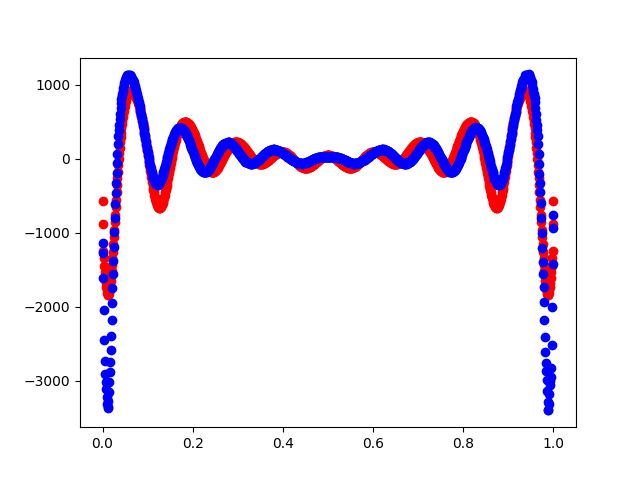
\includegraphics[width=6cm]{figure/example/model1_1000.png}
	\hspace{1cm}
	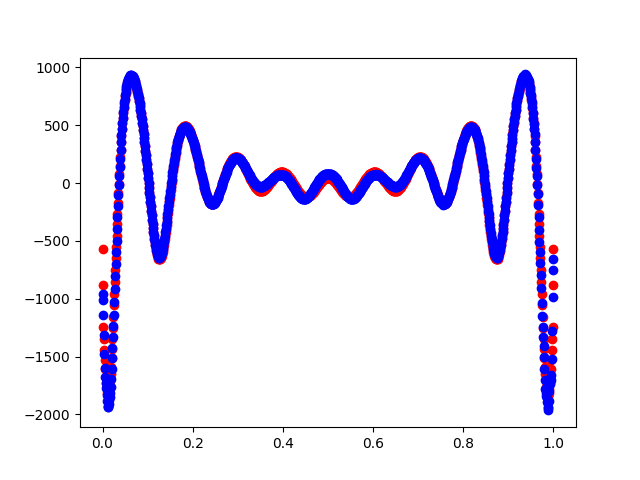
\includegraphics[width=6cm]{figure/example/model1_10000.png}
	\bicaption{中文题图}
	{English caption}
	\label{fig1}
\end{figure}

这里还有插入EPS图像和PDF图像的例子,如\autoref{fig2} 和\autoref{fig3}。这里将EPS和PDF图片作为子图插入,每个子图有自己的小标题。子图标题使用subcaption宏包添加。

\begin{figure}[htp]
	\centering
	\subcaptionbox{PDF 图像\label{fig2}}[3cm] %标题的长度,超过则会换行,如下一个小图。
	{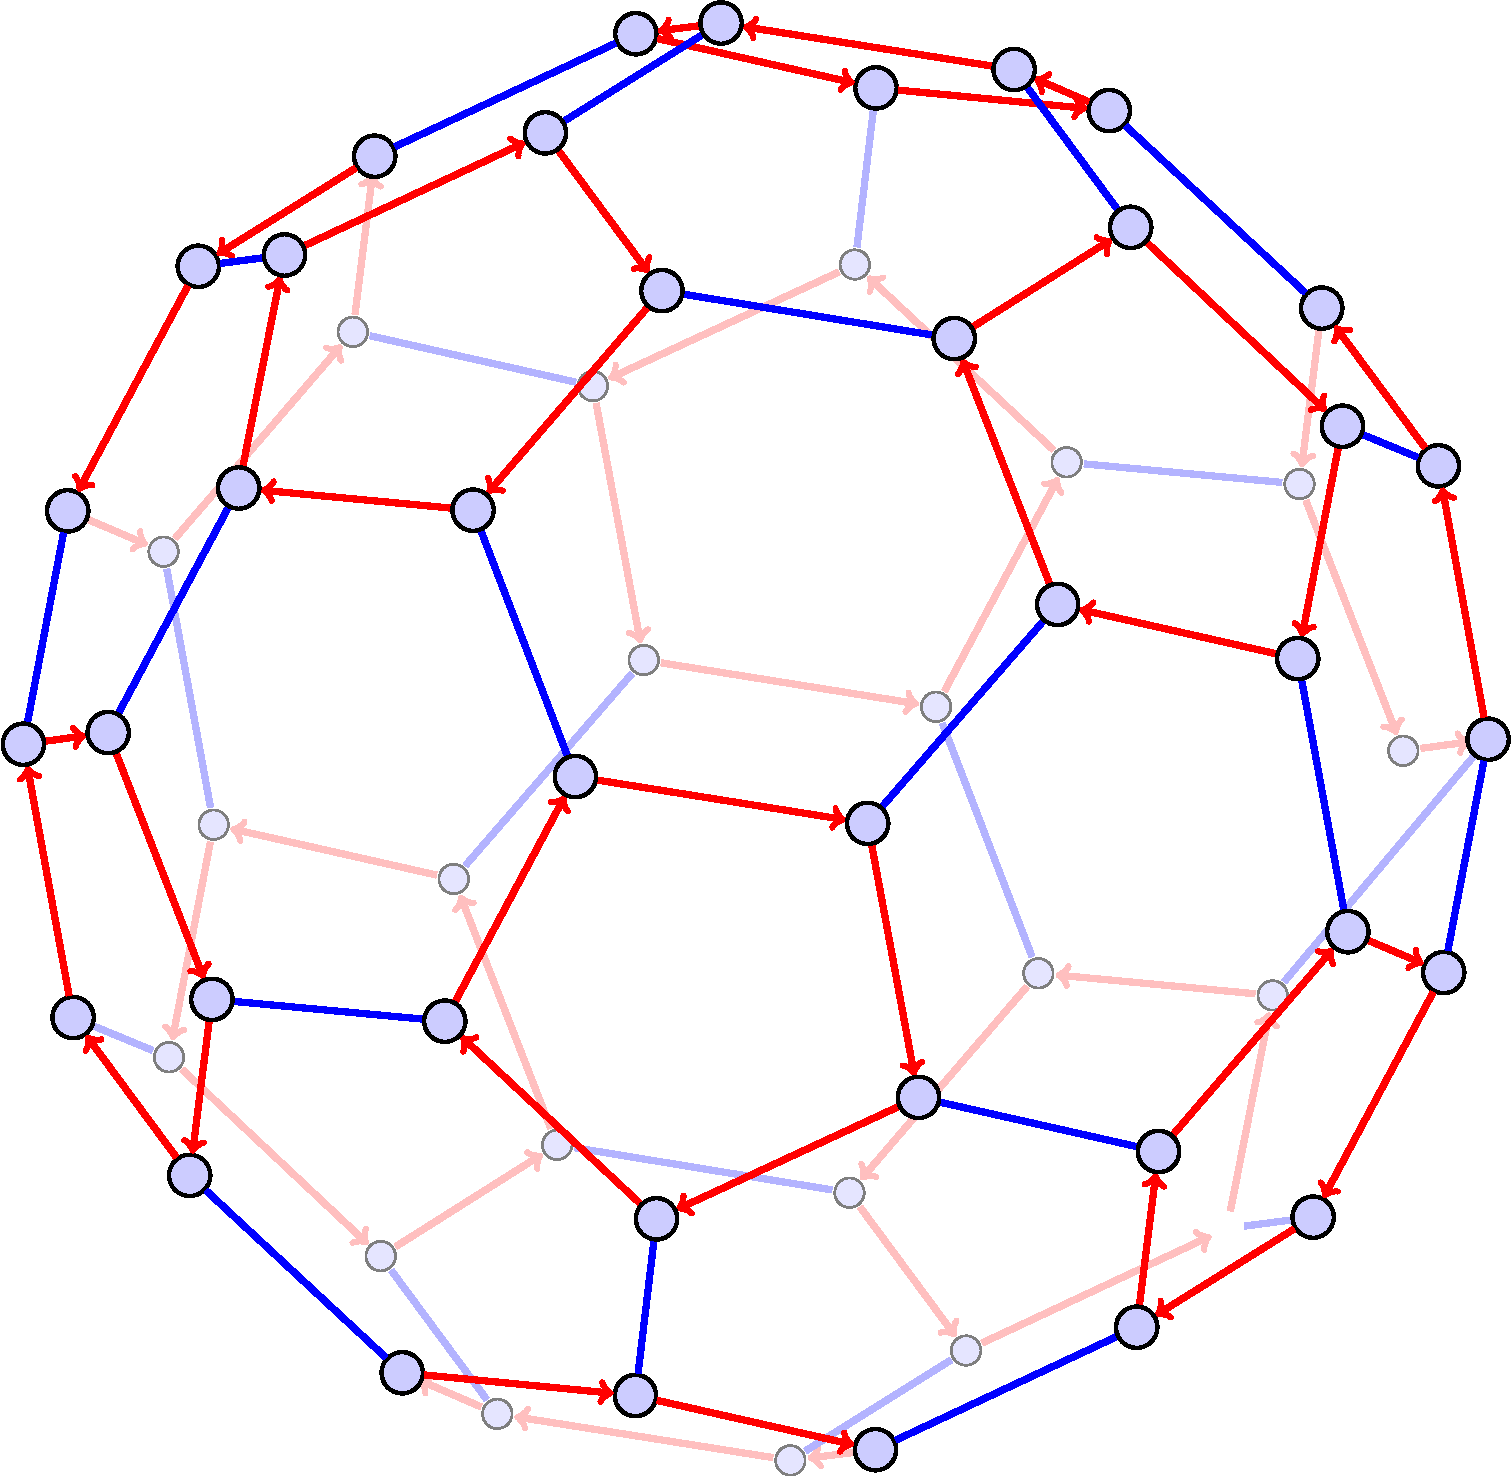
\includegraphics[height=2.5cm]{figure/example/m2.pdf}}
	\hspace{4em}
	\subcaptionbox{EPS 图像,如果标题很长的话,它会自动换行\label{fig3}}
	{	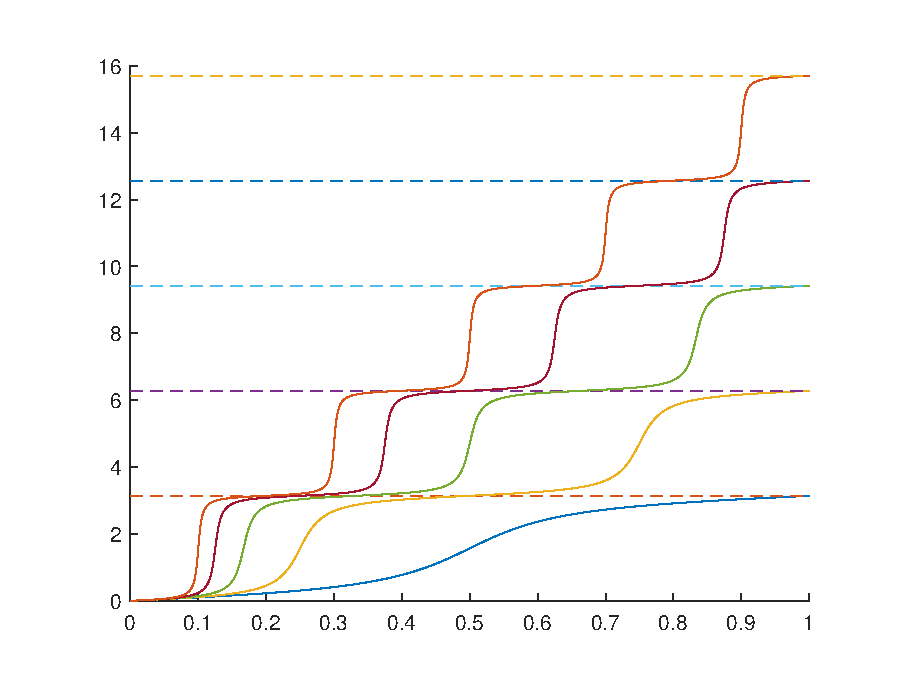
\includegraphics[scale=0.5]{figure/example/purfer_left.eps}}
	\bicaption{插入eps和pdf的例子(使用 subcaptionbox 方式)}{An EPS and PDF demo with subcaptionbox}
	\label{fig4}
\end{figure}。

\section{插入代码}

这里给一个使用listings宏包插入源代码的例子:
\begin{lstlisting}[language={C}, caption={一段C源代码}, label=code:1]
#include <stdio.h>

int main() {
    printf("Hello World!\n");
    return 0;
}
\end{lstlisting}
在\autoref{code:1}中,我们插入了一个C语言的Hello World代码。

\section{标签和引用}

这一节给出的是一些标签和引用的例子。

\subsection{标签设计原则}

为了更好的方便作者引用已经存在的标签,标签名必须见名知意。一般的设计原则是\verb|类型名:内容描述|。在\autoref{tab:typename} 中给出通常使用的类型的简称。

例如:\verb|thm:limit|,\verb|tab:typename|等等。

\begin{table}[!htp]
	\centering
	\caption{常见类型缩写}
	\begin{tabular}{c|c|c|c}\label{tab:typename}
		缩写 & 全称 & 缩写 & 全称 \\
		\hline
		part & part & fig & figure \\
		chap & chapter & tab & table \\
		sec & section & eq & equation \\
		subsec & subsection & algo & algorithm \\
		thm & theorem & def & definition \\
		lem & lemma & rem & remark \\
	\end{tabular}
\end{table}

\subsection{引用}

最简单的引用标签的方法就是使用\verb|\ref|命令,会显示被引用的定理(或者章节)对应的编号。
为了让文章可读性更强,我们通常会在\verb|\ref|命令前加入类型名,如\verb|<定理\ref{thm:telescope}>|。

\section{文献的添加和引用}

本模板的参考文献数据统一存放在\verb|bib/|目录下的\verb|ref.bib|文件中,如需添加文献,可以在INSPIRE HEP,百度学术,Google Scholar等界面查找到对应文献的\verb|bibtex|格式引用信息,然后附在\verb|ref.bib|文件末端即可。期刊,图书,学位论文的规范的\verb|bibtex|文献信息如下:
\begin{lstlisting}
@article{Sjostrand:2006za,
    author = "Sjostrand, Torbjorn and Mrenna, Stephen and Skands, Peter Z.",
    title = "{PYTHIA 6.4 Physics and Manual}",
    journal = "JHEP",
    volume = "05",
    number="15"
    pages = "026--029",
    year = "2006"
}
@book{zhang2020,
  author    = {张波 and 张景肖},
  title     = {应用随机过程},
  edition   = {1},
  publisher = {清华大学出版社},
  address   = {北京},
  year      = {2004},
  pages = {74--108},
}
@phdthesis {1015957626.nh,
author = { 张向华 },
title = {几类带Lévy跳的随机传染病模型的动力学性质分析},
address={哈尔滨},
school = {哈尔滨工业大学},
year = {2014}
}
\end{lstlisting}
第一行表明这个文献的类型是\verb|article|以及引用关键字为\verb|Sjostrand:2006za|。

文献添加后,如果需要引用,使用\verb|\cite{label}|命令即可,支持引用单个或多个文献。
演示如下:

命令\verb|\cite{Sjostrand:2006za}|的使用效果:在\cite{Sjostrand:2006za}中,作者已经阐述了有关结论。

命令\verb|\cite{bierlich2022comprehensive,王亚平2006}|的使用效果:在\cite{bierlich2022comprehensive,王亚平2006}中,作者有...

{\bf \textcolor{red}{重要提示}}:
如果在引用时发现不能正常显示引用标志的话,进入模板根目录下的\verb|cmd|环境,输入\verb|biber main|命令,然后再次编译即可。

% -*- coding=utf-8 -*-
\chapter{结论}
\songti\zihao{-4}
\linespread{1.67} \selectfont

这是结论。
    

 %正文章节

%========= 附录部分 =========
\backmatter

% -*- coding=utf-8 -*-
%\nocite{*}显示未引用的参考文献
\printbibliography[title=参考文献,heading=bibintoc]

%% -*- coding=utf-8 -*-
\chapter{附录}

% -*- coding=utf-8 -*-
\chapter{致谢}
大学本科生活结束了。







\end{document}
